\documentclass[11pt]{article}

\usepackage[spanish]{babel}
\usepackage[utf8]{inputenc}
\usepackage[T1]{fontenc}
\usepackage[margin=2.5cm]{geometry}
\usepackage{graphicx}
\usepackage{booktabs}
\usepackage{caption}
\usepackage{float}
\usepackage[hidelinks]{hyperref}

\setlength{\parindent}{1.5em}
\setlength{\parskip}{0pt}

\begin{document}

\begin{center}
{\LARGE Laboratorio 6: An\'alisis de redes sociales en YouTube}\\[4pt]
{\large CC3084 -- Data Science, Semestre II 2026}
\end{center}

\vspace{0.8cm}

\begin{center}
Anthony Lou Schwank -- 23410 \\
Isabella Obando -- 23074 \\
Francisco Martinez -- 23617
\end{center}

\vspace{0.5cm}

\begin{center}
Repositorio del proyecto:\\
\texttt{https://github.com/anthonylouschwank/Lab6-DS}
\end{center}

\vspace{0.5cm}

\section{Introducci\'on}

El objetivo del laboratorio fue estudiar la estructura de participaci\'on de
usuarios en YouTube a partir de dos conjuntos de datos: \texttt{youtube\_videos.csv}
(293 videos de canales guatemaltecos) y \texttt{youtube\_comments.csv} (406
comentarios). El trabajo combin\'o limpieza de datos, an\'alisis exploratorio,
construcci\'on y an\'alisis de redes (bipartita autor-video, proyecciones,
comunidades, centralidad) y an\'alisis de sentimiento de texto en espa\~nol. Todo el
c\'odigo est\'a organizado en \texttt{src/} (\texttt{p1\_load\_integrate.py} a
\texttt{p9\_sentiment.py}, ejecutables en orden con \texttt{python src/run\_all.py}),
con tablas en \texttt{outputs/tables/} y figuras en \texttt{outputs/figures/}.

\section{Descripci\'on e integraci\'on de los datos}

Cada fila de \texttt{youtube\_videos.csv} es un video (llave primaria
\texttt{video\_id}) y cada fila de \texttt{youtube\_comments.csv} es un comentario
principal (llave primaria \texttt{comment\_id}, con \texttt{video\_id} como llave
for\'anea y \texttt{author\_channel\_id} como identificador del autor). La relaci\'on
canal-video es 1 a N, video-comentario es 1 a N, y autor-video es \textbf{N a N}
--es justamente esta \'ultima la que se modela como red bipartita m\'as adelante.

Al integrar ambos conjuntos por \texttt{video\_id}, el 100\% de los 406 comentarios
se asocia correctamente a un video, pero esos comentarios se concentran en solo
\textbf{19 de los 293 videos (6.5\%)}. No es un error de integraci\'on sino del
procedimiento de recolecci\'on: los comentarios solo se extrajeron para una
selecci\'on de videos. Este hallazgo condiciona todo el resto del an\'alisis: la red,
la concentraci\'on de participaci\'on y el sentimiento se refieren a esos 19 videos y
a los 332 autores que comentaron en ellos, no al corpus completo.

\section{Limpieza y preprocesamiento}

El diagn\'ostico de calidad no encontr\'o duplicados (0 \texttt{video\_id} ni
\texttt{comment\_id} repetidos) y confirm\'o consistencia total entre identificadores
y nombres visibles (todo \texttt{channel\_id}/\texttt{author\_channel\_id} mapea a un
\'unico nombre). Se identificaron variables in\'utiles o delicadas: \texttt{viewer\_rating}
(100\% vac\'ia, se descarta), \texttt{is\_pinned} (constante), \texttt{upload\_date} y
\texttt{owner\_handle} (redundantes con otras columnas), y \texttt{reply\_count}, que
--como aclara el enunciado-- \textbf{no identifica a los autores de las respuestas},
por lo que nunca se us\'o para construir aristas autor-autor.

Los conteos guardados como texto se convirtieron a n\'umero (\texttt{like\_count\_text},
46.6\% vac\'io, interpretado como 0 ``me gusta'' visibles, el comportamiento normal de
la interfaz de YouTube). Se conservaron dos versiones del texto de cada comentario:
\texttt{texto\_original} (intacto, para el an\'alisis de sentimiento) y
\texttt{texto\_limpio}, que aplica min\'usculas, elimina URLs, separa menciones y
hashtags a columnas propias, convierte emojis a su descripci\'on en espa\~nol (en vez
de borrarlos, porque son la principal se\~nal de sentimiento en comentarios cortos),
quita acentos, puntuaci\'on y \emph{stopwords} en espa\~nol. No se lematiz\'o: con
comentarios tan cortos, un lematizador ligero pod\'ia introducir m\'as errores
gramaticales que beneficio. El efecto neto de la limpieza fue modesto: 0 textos
originales vac\'ios, solo 1 texto limpio vac\'io, y una reducci\'on de 139 a 100
caracteres promedio.

\section{An\'alisis exploratorio}

La participaci\'on est\'a fuertemente concentrada: un solo video (\emph{``Qu\'e rico
come tu diputado''}, canal Quorum) re\'une el \textbf{39.7\%} de los 406 comentarios,
y el canal Quorum por s\'i solo explica el \textbf{63.1\%}, con solo 11 de los 293
videos del conjunto completo (Figura~\ref{fig:comentarios_video}). Las
visualizaciones de los 293 videos tienen una distribuci\'on much\'isimo m\'as sesgada
(m\'inimo 2, mediana 1{,}175, m\'aximo 8{,}190{,}449).

\begin{figure}[H]
\centering
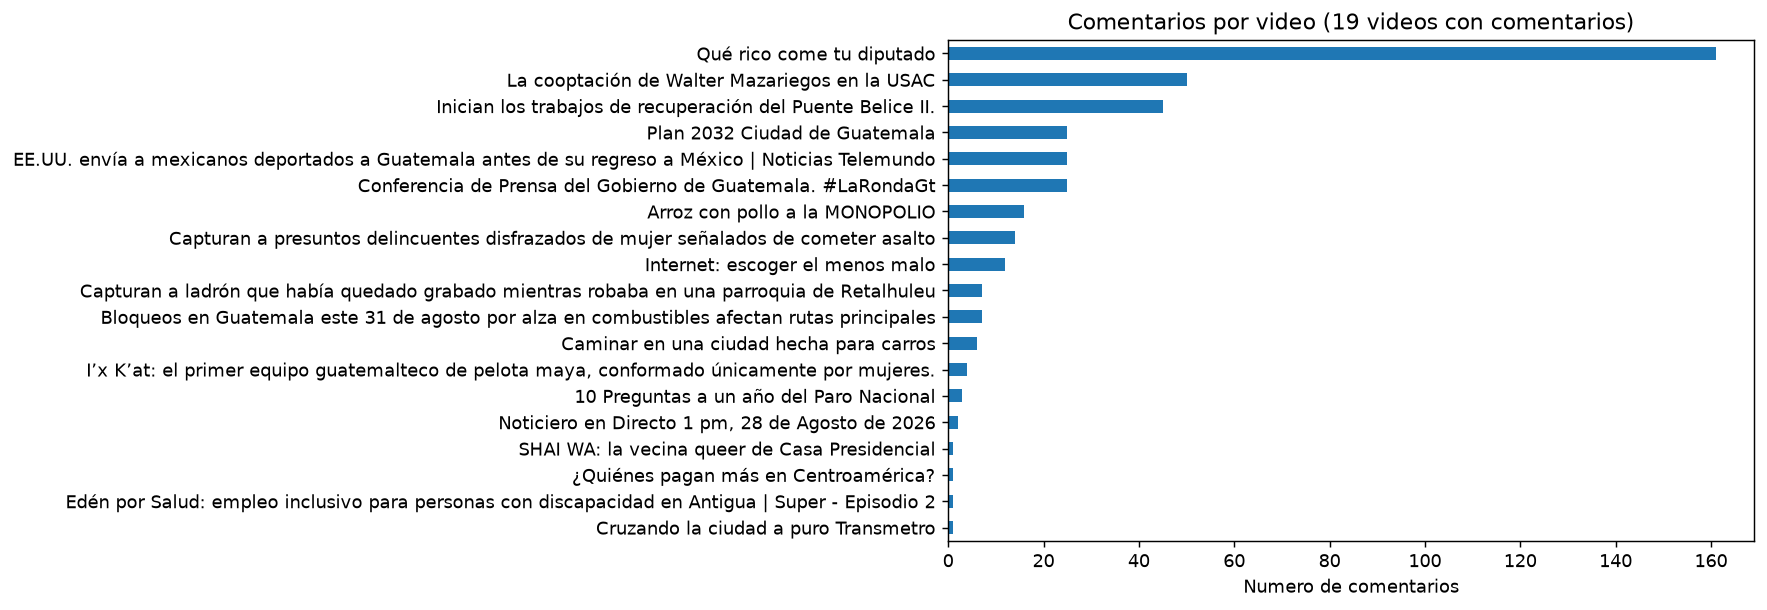
\includegraphics[width=0.85\textwidth]{../outputs/figures/03_comentarios_por_video.png}
\caption{Comentarios por video (los 19 videos con comentarios en la muestra).}
\label{fig:comentarios_video}
\end{figure}

Entre popularidad y participaci\'on hay una correlaci\'on de Spearman positiva y
fuerte ($\rho = 0.811$) para esos 19 videos, pero no es monot\'onica: el video m\'as
visto de la submuestra (\textasciitilde304{,}000 vistas, un video institucional de la
Municipalidad) recibi\'o solo 25 comentarios, mientras que el m\'as comentado (161)
apenas tiene \textasciitilde11{,}800. El tipo de contenido (opini\'on/humor vs.
comunicado institucional) parece importar tanto como el alcance bruto.

Un hallazgo notable del an\'alisis de frecuencias es que buena parte de los bigramas
m\'as frecuentes de \texttt{texto\_limpio} son en realidad \textbf{emojis convertidos a
texto} (\emph{cara llorando}, \emph{manos aplaudiendo}, \emph{bandera guatemala},
Figura~\ref{fig:bigramas}): una fracci\'on relevante del ``contenido textual'' es
reacci\'on emotiva breve, no argumento desarrollado. Las palabras sueltas con
contenido tem\'atico genuino (\emph{pueblo}, \emph{dinero}, \emph{diputados},
\emph{corruptos}) apuntan a cr\'itica pol\'itico-econ\'omica. De los 332 autores,
solo \textbf{9 comentaron en m\'as de un video} (2.7\%); de ellos, 7 comparten
audiencia dentro del mismo canal y solo 2 cruzan de canal.

\begin{figure}[H]
\centering
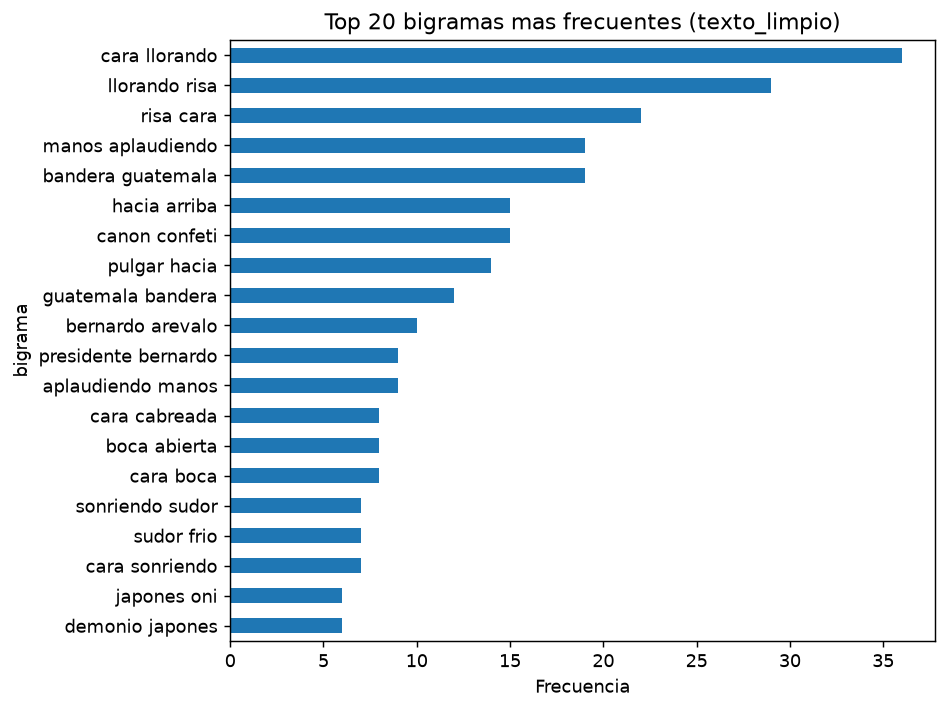
\includegraphics[width=0.85\textwidth]{../outputs/figures/03_top_bigramas.png}
\caption{Bigramas m\'as frecuentes en \texttt{texto\_limpio}: n\'otese cu\'antos provienen de emojis.}
\label{fig:bigramas}
\end{figure}

\section{Red bipartita autor-video}

Se construy\'o una red bipartita no dirigida (\texttt{networkx}) con dos tipos de
nodo: 19 \textbf{videos} y 332 \textbf{autores}. Existe una arista si el autor
coment\'o en el video, con peso igual al n\'umero de comentarios que dej\'o ah\'i
(agregando repeticiones). El resultado son \textbf{351 nodos y 343 aristas}
(Figura~\ref{fig:bipartita}), con 40 aristas de peso mayor a 1. Una arista indica
\'unicamente co-presencia de comentarios: \textbf{no} implica que dos autores
conectados al mismo video se conozcan o est\'en de acuerdo, ni que el autor haya
visto el video completo, y --siguiendo la aclaraci\'on expl\'icita del enunciado--
\texttt{reply\_count} nunca se interpret\'o como arista, porque no identifica a
qui\'en respondi\'o.

\begin{figure}[H]
\centering
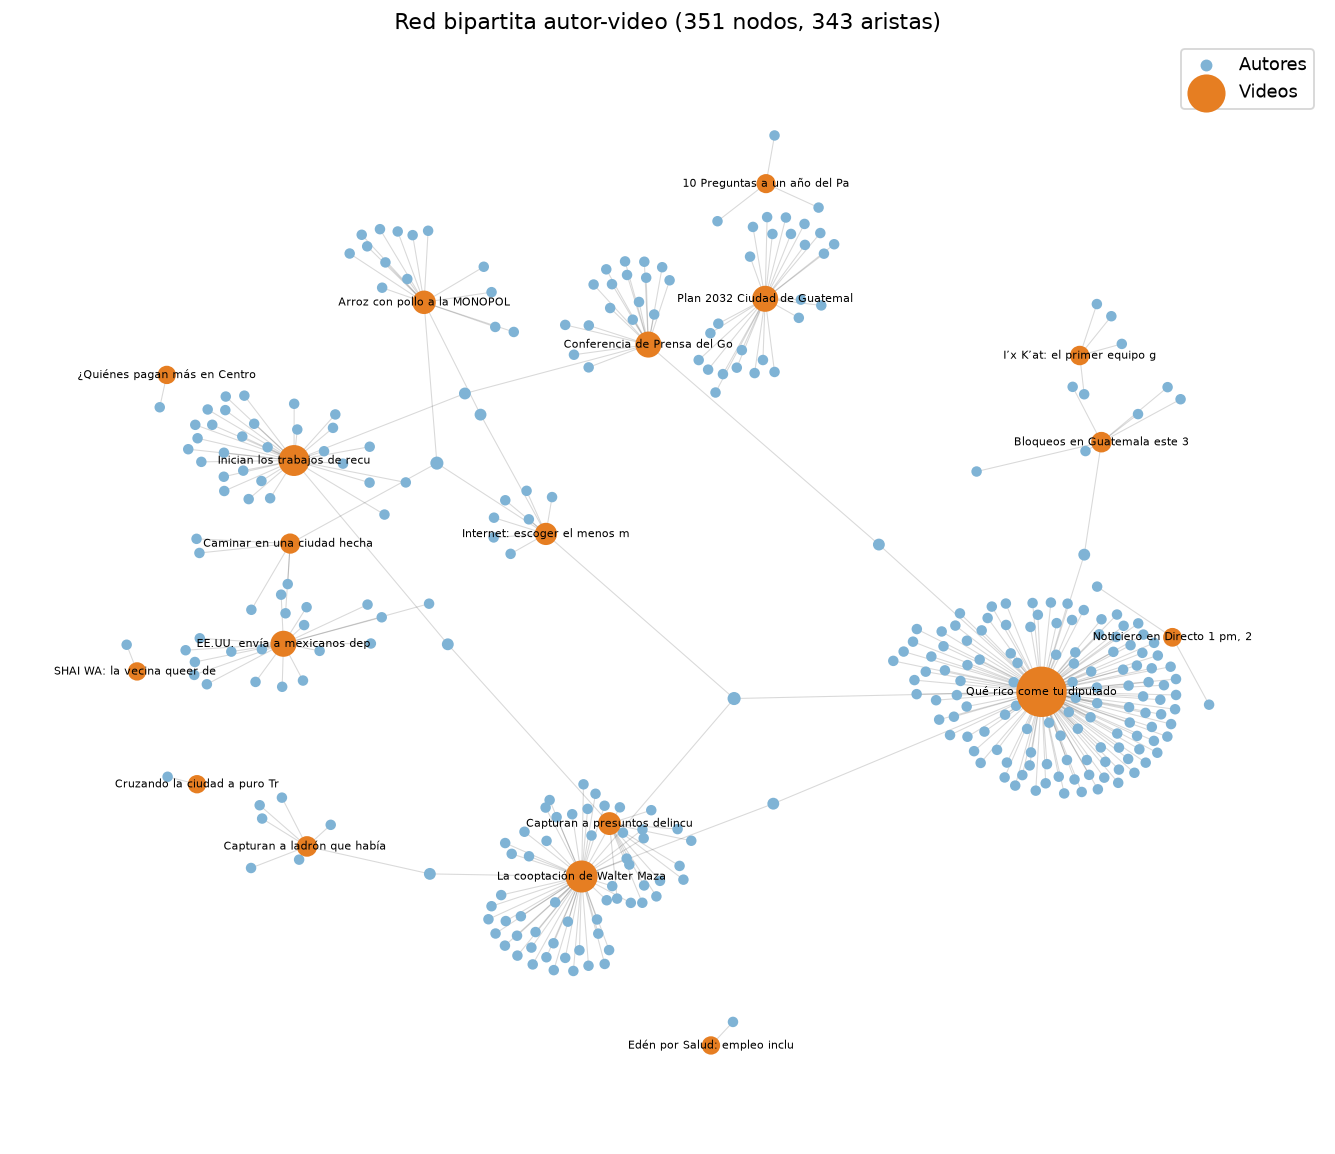
\includegraphics[width=0.85\textwidth]{../outputs/figures/04_red_bipartita.png}
\caption{Red bipartita completa autor-video (351 nodos, 343 aristas, sin podar).}
\label{fig:bipartita}
\end{figure}

\section{Proyecciones y topolog\'ia de la red}

A partir de la bipartita se construyeron dos proyecciones ponderadas: \textbf{autor-autor}
(arista si comparten un video, peso = videos compartidos) y \textbf{video-video}
(arista si comparten un autor, peso = autores compartidos). La primera crece a
\textbf{332 nodos y 10{,}732 aristas}: un video con 128 comentaristas genera por s\'i
solo miles de conexiones ``todos contra todos'', por lo que su altísima transitividad
(0.984) es en gran parte un artefacto de la proyecci\'on, no evidencia de un grupo
social cohesionado. La segunda, mucho m\'as parca (\textbf{19 nodos, 11 aristas},
Figura~\ref{fig:proyeccion_video}), es m\'as informativa: identifica qu\'e videos
comparten audiencia real, y muestra que \textbf{9 de los 19 videos quedan totalmente
aislados} (ning\'un autor en com\'un con otro), mientras que los 10 restantes forman
una \'unica componente conectada gracias a solo 9 autores puente.

\begin{figure}[H]
\centering
\includegraphics[width=0.7\textwidth]{../outputs/figures/05_video_projection.png}
\caption{Proyecci\'on video-video: 19 nodos, 11 aristas.}
\label{fig:proyeccion_video}
\end{figure}

La Tabla~\ref{tab:topologia} resume la topolog\'ia de las tres redes. Las tres
comparten la misma fragmentaci\'on de fondo (10 componentes), y en la bipartita el
93\% de los nodos tiene grado 1: la enorme mayor\'ia de los autores coment\'o una sola
vez en un solo video. Este aislamiento es \emph{observado}, no necesariamente real:
esos autores podr\'ian participar en muchos otros videos fuera de esta muestra de 406
comentarios.

\begin{table}[H]
\centering
\caption{M\'etricas de topolog\'ia por red.}
\label{tab:topologia}
\begin{tabular}{lrrrrr}
\toprule
Red & Nodos & Aristas & Densidad & Componentes & Comp. mayor \\
\midrule
Bipartita & 351 & 343 & 0.0056 & 10 & 286 (81.5\%) \\
Autor-autor & 332 & 10{,}732 & 0.1953 & 10 & 276 (83.1\%) \\
Video-video & 19 & 11 & 0.0643 & 10 & 10 (52.6\%) \\
\bottomrule
\end{tabular}
\end{table}

\section{Comunidades}

Se aplic\'o \textbf{Louvain ponderado} (\texttt{networkx.community.louvain\_communities},
semilla fija 42) sobre la proyecci\'on video-video, por ser la red m\'as peque\~na y
la que representa directamente audiencia compartida entre contenidos (la
autor-autor, dominada por cliques de proyecci\'on, habr\'ia redescubierto solo ``qui\'en
coment\'o en cu\'al video''). El algoritmo encontr\'o \textbf{12 comunidades} con
modularidad $Q = 0.4053$, aunque 9 de ellas son videos aislados sin ninguna arista
(comunidades triviales de un nodo). Las tres comunidades no triviales, dentro de la
componente de 10 videos, se resumen en la Tabla~\ref{tab:comunidades} y se
visualizan en la Figura~\ref{fig:comunidades}.

\begin{table}[H]
\centering
\caption{Las tres comunidades principales de la proyecci\'on video-video.}
\label{tab:comunidades}
\begin{tabular}{lrrrl}
\toprule
Comunidad & Videos & Comentarios & \% del total & Tema dominante \\
\midrule
1 & 4 & 225 & 55.4\% & Cr\'itica a diputados y corrupci\'on \\
2 & 3 & 84 & 20.7\% & Reacci\'on a figuras y anuncios de gobierno \\
3 & 3 & 34 & 8.4\% & Pol\'itica de telecomunicaciones/mercado \\
\bottomrule
\end{tabular}
\end{table}

\begin{figure}[H]
\centering
\includegraphics[width=0.85\textwidth]{../outputs/figures/07_video_communities.png}
\caption{Comunidades de la proyecci\'on video-video (Louvain, $Q=0.4053$).}
\label{fig:comunidades}
\end{figure}

\section{Centralidad y nodos puente}

Sobre la bipartita se calcularon grado, fuerza (grado ponderado), intermediaci\'on
(\emph{betweenness}) y PageRank; se complement\'o con puntos de articulaci\'on
(\texttt{nx.articulation\_points}), que responden con precisi\'on a ``si elimino este
nodo, \textquestiondown se segmenta la red?''. No se us\'o cercan\'ia por la
fragmentaci\'on en 10 componentes, donde esa m\'etrica deja de ser comparable.

El resultado matiza el hallazgo del EDA: de los 9 autores con comentarios en m\'as de
un video, solo \textbf{7 son puntos de articulaci\'on reales} (su remoci\'on
fragmenta la red); los otros 2 conectan pares de videos que ya comparten otro puente
redundante, por lo que quitarlos individualmente no desconecta nada. En el lado de
los videos, 15 de los 19 muestran intermediaci\'on mayor a 0, pero en su mayor\'ia de
forma trivial (son el \'unico camino entre sus propios comentaristas, que no est\'an
conectados entre s\'i de otro modo); solo los que adem\'as participan en la componente
de 10 conectan audiencias realmente distintas. En conjunto, la mitad de los videos
con comentarios permanece unida a la otra mitad gracias, en \'ultima instancia, a un
n\'ucleo de solo 7 personas.

\section{An\'alisis de sentimiento}

Se us\'o \textbf{pysentimiento} con \textbf{RoBERTuito}, un modelo tipo RoBERTa
preentrenado y afinado sobre tuits en espa\~nol~\cite{robertuito2021}, preferido sobre
un l\'exico simple porque nuestros comentarios son cortos, informales y con emojis
convertidos a texto --exactamente el dominio para el que RoBERTuito fue entrenado-- y
porque capta negaci\'on y contexto mejor que sumar polaridad palabra por palabra. El
an\'alisis corri\'o sobre \texttt{texto\_original}, no sobre \texttt{texto\_limpio},
para no perder las se\~nales (acentos, may\'usculas, formato del emoji) que el modelo
usa.

El sentimiento global es \textbf{61.3\% negativo, 19.5\% neutro y 19.2\% positivo}
(Figura~\ref{fig:sentimiento_global}), coherente con el vocabulario de cr\'itica
pol\'itico-econ\'omica ya identificado. Pero no es uniforme: como muestra la
Figura~\ref{fig:sentimiento_video}, \emph{``Plan 2032 Ciudad de Guatemala''} (un video
institucional de la Municipalidad) es un outlier claro con \textbf{80\% de
sentimiento positivo}, mientras que videos de cr\'itica pol\'itica superan 80\%
negativo. Esto sugiere que el sentimiento responde m\'as al \emph{tipo de evento
narrado} (denuncia/corrupci\'on vs. anuncio de obra) que a un sesgo generalizado en
contra de alg\'un canal en particular --de hecho, otros videos del propio Gobierno de
Guatemala caen del lado negativo.

\begin{figure}[H]
\centering
\includegraphics[width=0.55\textwidth]{../outputs/figures/09_sentiment_global.png}
\caption{Distribuci\'on global de sentimiento (406 comentarios).}
\label{fig:sentimiento_global}
\end{figure}

\begin{figure}[H]
\centering
\includegraphics[width=0.85\textwidth]{../outputs/figures/09_sentiment_by_video.png}
\caption{Sentimiento por video (videos con al menos 5 comentarios).}
\label{fig:sentimiento_video}
\end{figure}

\section{Limitaciones}

Solo el 6.5\% de los videos (19/293) tiene comentarios en la muestra, y no fueron
elegidos al azar sino mediante consultas de b\'usqueda dirigidas
(\texttt{source\_query}/\texttt{source\_group}), lo que sobre-representa a un canal de
opini\'on (Quorum explica 63\% de los comentarios) frente al resto del corpus. Las
fechas de publicaci\'on de los comentarios son relativas (``hace 2 d\'ias'') y
dependen del momento de la recolecci\'on, por lo que no se puede reconstruir una
l\'inea de tiempo exacta. Los conteos de vistas y ``me gusta'' son una fotograf\'ia de
un \'unico momento, no valores estables. Finalmente, \texttt{reply\_count} no
identifica autores de respuestas, as\'i que toda la red se basa \'unicamente en
comentarios principales, no en hilos de conversaci\'on reales; y buena parte de las
m\'etricas de red dependen de un solo video (161/406 comentarios) y de apenas 7
autores puente, por lo que son sensibles a cambios peque\~nos en esos pocos nodos.

\section{Conclusiones}

Dentro de esta muestra, la conversaci\'on de YouTube alrededor de contenido
guatemalteco es estructuralmente fragmentada (la mitad de los videos con comentarios
no comparte ning\'un autor con el resto) pero muy concentrada dentro de su componente
principal, con la conectividad entre videos sostenida por muy pocas personas. Es
tambi\'en tem\'aticamente polarizada hacia la cr\'itica pol\'itico-econ\'omica, con un
sentimiento global 61.3\% negativo, aunque esa negatividad depende m\'as del
\emph{g\'enero} del video (denuncia vs. anuncio institucional) que de qui\'en lo
public\'o. Dado que un solo canal explica el 63\% de los comentarios analizados y que
la selecci\'on de videos no fue aleatoria, estos resultados deben leerse como una
fotograf\'ia descriptiva de esta muestra puntual, \'util para entender la din\'amica de
participaci\'on dentro de estos 19 videos, y no como evidencia representativa del
consumo de YouTube en Guatemala en general.

\begin{thebibliography}{9}
\bibitem{networkx}
Hagberg, A., Swart, P., \& Chult, D. (2008). Exploring Network Structure, Dynamics,
and Function using NetworkX. \emph{Proceedings of the 7th Python in Science
Conference (SciPy2008)}.

\bibitem{louvain}
Blondel, V. D., Guillaume, J.-L., Lambiotte, R., \& Lefebvre, E. (2008). Fast
unfolding of communities in large networks. \emph{Journal of Statistical Mechanics}.

\bibitem{robertuito2021}
P\'erez, J. M., Furman, D. A., Alonso Alemany, L., \& Luque, F. (2021). RoBERTuito: a
pre-trained language model for social media text in Spanish. \emph{arXiv:2111.09453}.

\bibitem{nltk}
Bird, S., Klein, E., \& Loper, E. (2009). \emph{Natural Language Processing with
Python}. O'Reilly Media.
\end{thebibliography}

\end{document}
